% !TeX encoding = UTF-8
% !TeX spellcheck = en_US

\documentclass[
	paper=A4,
	parskip=full,
	chapterprefix=true,
	11pt,
	headings=normal,
	bibliography=totoc,
	listof=totoc,
	titlepage=on,
]{scrreprt}

\usepackage{../../lieb}

\usepackage{feynmp}
\DeclareGraphicsRule{.1}{mps}{*}{}

\graphicspath {{../images/}}

\heads{RWTH Aachen \\ Particlephyics Lab}{T17 \\ W-Boson}{Lieb | Stettner \\ \today} 
\date{\today}

\newcommand{\MET}{\ensuremath{{\slashed{E}_\mathrm{T}}}\xspace}
\newcommand{\ELET}{\ensuremath{{E_\mathrm{T}^\mathrm{el}}}\xspace}

\newcommand{\thirdwidth}{0.32\textwidth}
\newcommand{\halfwidth}{0.48\textwidth}
\newcommand{\fullwidth}{1.0\textwidth}

\setlength\parindent{0pt}
\setlength{\parskip}\medskipamount

\title{Particle Physics Laboratory Class \\ \quad \\ Experiment T17 | W-Boson }
\author{Jonas Lieb (312136) \\ Jöran Stettner (312169) \\ \\  RWTH Aachen}

\newcommand{\dnull}{D$\slashed{\mathrm{0}}$\xspace}

\begin{document}

\maketitle

\cleardoublepage

\setcounter{tocdepth}{2}
\tableofcontents

\cleardoublepage

\chapter{Introduction}

This analysis deals with \PW boson physics conducted at the \dnull experiment at the Tevatron accelerator (FERMILAB, Chicago). The data has been taken in proton-antiproton collisions at a center-of-mass energy of $\sqrt{s} = \SI{1960}{\giga\electronvolt}$.

\section{Units}
In this report, a natural unit system of particle physics is used: first, the speed of light and Planck's constant are fixed:
\begin{equation}
c \defeq \num{1},\quad \hbar \defeq \num{1}
\end{equation}
From this convention, many quantities arise in units of energy. Additionally, the gigaelectronvolt (\si{\giga\electronvolt}) is chosen as basic energy unit, in order to deal with numbers of magnitude $\order{1}$.

\section{\PW Boson Production and Decay}
The process of interest is the \PW boson production from the valence quarks of the protons and antiprotons, and the decay into an electron and an electron neutrino.
\begin{equation}
	\Pproton\APproton \rightarrow \PWminus \rightarrow \Pelectron \APnue
\end{equation}
Equivalently, there exists a oppositely charged process:
\begin{equation}
\Pproton\APproton \rightarrow \PWplus \rightarrow \Ppositron \Pnue
\end{equation}
With the assumption that the \PWplus and \PWminus have similar properties (except the electric charge), one does not expect any difference between the processes. Because of that, the analysis will not differentiate between them and treat positrons as electrons in the final state.

Both processes combined have an expected cross section\cite{HBK+2013Experiment} of 
\begin{equation}
	\sigma_\mathrm{theo} = \SI{2.58 +- 0.09}{\nano\barn}
	\label{eq:theoretical_cross_section}
\end{equation}
and should show a resonance at the predicted \PW-Boson mass\cite{Oo2014Review} of 
\begin{equation}
	m_{\PW} = \SI{80.385 +- 0.015}{\giga\electronvolt}
\end{equation}

\section{The \dnull Detector}
The measurement took place in 2004 until 2006 at the \dnull experiment at FERMILAB. The \dnull detector is a cylindrical particle detector located around the Tevatron beam pipe. It consist of a silicon tracker in the center region, enclosed by an Argon electromagnetic calorimeter.

Inside the detector, a Cartesian coordinate system and a cylindrical coordinate system are used. The origin of both systems lies in the interaction point, with the z-axis pointing along the beam pipe. The angle $\phi$ is measured in a plane perpendicular to the z-axis. 

Because the colliding protons are composite particles, the longitudinal momentum of the interacting quarks is unknown. The transversal components, however, are zero in the initial state. From momentum conservation it follows that the sum of all transversal momenta in the final state is also zero. 
To represent this conservation in the transversal plane, energies and momenta are projected onto it. This introduces the transverse electron energy \ELET.
Another important definition is the missing transverse energy \MET which is calculated as negative sum of all particles momenta, projected onto the transverse plane.


\chapter{Monte-Carlo Samples}
\label{ch:mc_samples}

\section{Reweighting}
The final goal of this experiment is to perform a template fit between distributions of Monte Carlo (MC) simulated events and measured data, in order to find the \PW-Boson mass $m_{\PW}$. For the template fit, multiple MC distributions are necessary, one for each hypothetical \PW boson mass. Since MC simulations are computation intensive, an alternative approach is used: the actual simulation has only been performed once, but each MC event additionally contains a set of \num{19} weights, which correspond to different hypothetical \PW masses in the range of \SIrange{79.9446}{80.8446}{\giga\electronvolt} (for a complete reference, see the appendix of \cite{HBK+2013Experiment}). When aggregating distributions, each event has to be counted with the weight of the \PW mass of interest.

\begin{figure}
	\centering
	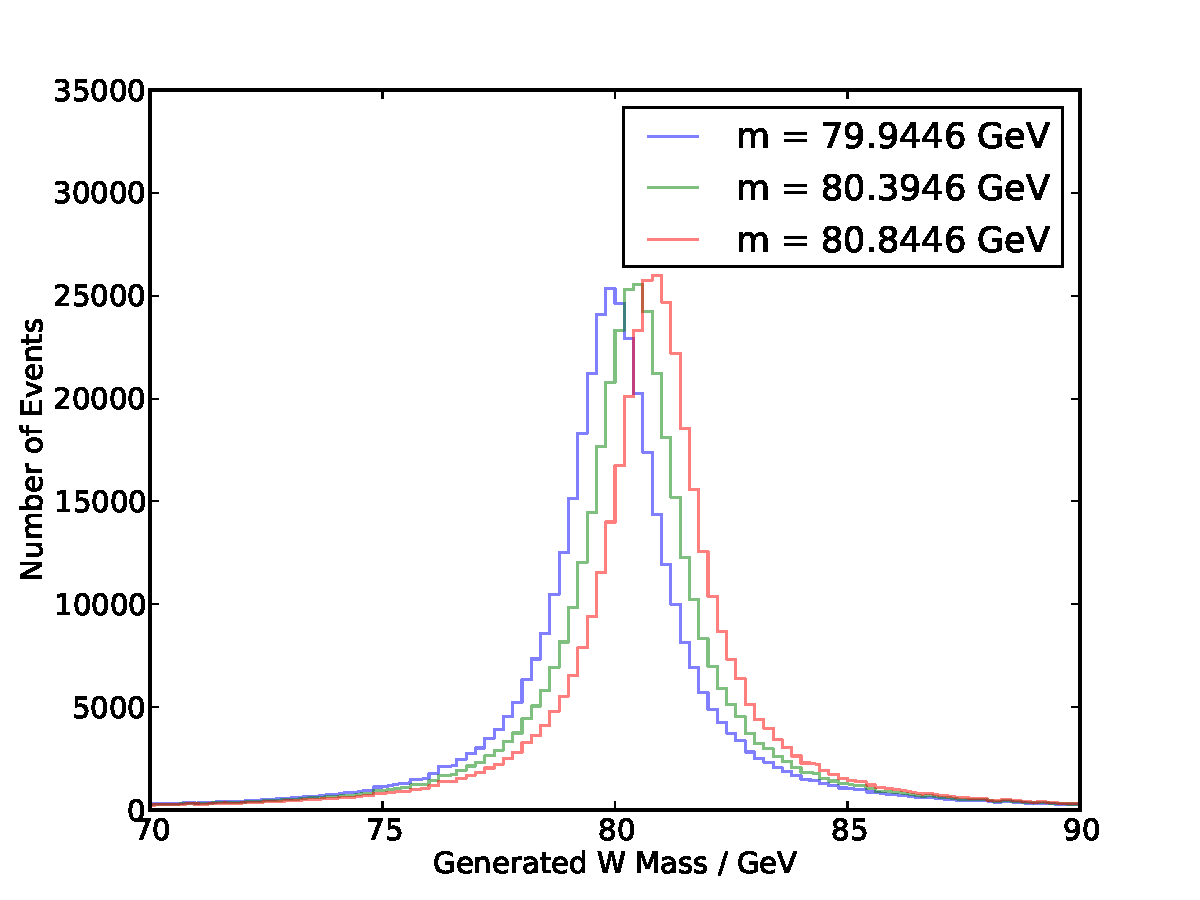
\includegraphics{mc_examples}
	\caption{Histogram of \PW masses. Shown is the generator W mass, which is stored inside the MC events, reweighted for three different example masses. One can observe the expected Breit-Wigner distribution, with the centers shifted.}
	\label{fig:mc_examples}
\end{figure}

Figure \ref{fig:mc_examples} shows the result of reweighting for example values. For this plot, the "true" \PW mass has been obtained from the Monte Carlo generator data. The histogram has been filled with the generator mass and the weighs corresponding to the \PW masses \SI{79.9446}{\giga\electronvolt}, \SI{80.3946}{\giga\electronvolt} and \SI{80.8446}{\giga\electronvolt}. The illustration shows that the reweighting approach is valid, although the weights only change the plot along the vertical axis, the overall Breit-Wigner curve has shifted to different masses.

\section{Scaling}
Only a limited amount of measured data is available. Its integrated luminosity of the data sample\cite{HBK+2013Experiment} is:
\begin{equation}
	\mathcal{L_\mathrm{data}} = \SI{198 +- 20}{\per\pico\barn}
\end{equation}
Opposed to this, only $N_\mathrm{gen} = \num{1164699}$ Monte Carlo events have been generated. An intuitive way to match the number of MC events to the number of data events is to construct a "MC luminosity". For this, the theoretical cross section from equation \ref{eq:theoretical_cross_section} is used:
\begin{equation}
	\mathcal{L_\mathrm{MC}} = \frac{N_\mathrm{gen}}{\sigma_\mathrm{theo}} = \SI{451 +- 16}{\per\pico\barn}
\end{equation}
This shows that the number of MC events has to be scaled down by a factor of about \num{2.3}. Curiously enough, the lab manual suggests an additional correction factor of $\mathrm{corr} = \num{0.90 +- 0.10}$.
Thus, the complete weight for each MC event (not including the shape-reweighting) is:
\begin{equation}
	w = \frac{\mathcal{L_\mathrm{data}}}{\mathcal{L_\mathrm{MC}}} \cdot (\num{0.90 +- 0.01}) = \num{0.40 +- 0.06}
\end{equation}


\chapter{Selection of Events}
In this chapter, the measured variables are presented and the selection of events is explained. \\
The distributions of the measured and simulated quantities are shown in figures \ref{fig:no_cuts_Etmet}, \ref{fig:no_cuts_etadphi} and \ref{fig:no_cuts_dziso}. The histogram labeled 'MC' contains all simulated events but the small component of $\tau$-leptons is plotted separately to point out it's contribution. It becomes clear that the MC-generator did not simulate all processes which occur in the detector, see for example the double-bump structure in the distribution of transverse electron energy. To perform the analysis as sketched above, it is important to select only those events which fall in regions where data and MC are in good agreement. Otherwise, a discrepancy coming from background processes or missing simulation would be interpreted as a mismatch to the simulated W-mass. Among others, occuring background processes are: 
\begin{itemize}
	\item $\Ppizero \rightarrow 2 \Pphoton$ decays which could account for the lower electron energies if the $\gamma$ is misidentified.
	\item Jets which are misidentified as electrons. The electron isolation variable becomes smaller in this case.
	\item $\PZ \rightarrow \Ppositron \Pelectron$ decays where one of the leptons leaves the detector unnoticed.
	\item $\tau \rightarrow e+\bar{\nu_e}+\nu_{\tau}$ (also simulated in MC)
\end{itemize}

To constrain the analysis to regions of good agreement between MC and data, the following cuts are applied to all events:
\begin{table}[htbp]
	\centering
	\begin{tabular}{ 
			l 
			l
			l
			l
		}
		\toprule
		{Quantity} & {Threshold} & { } \\ 
		\midrule
		\MET & $>\SI{20}{\giga\electronvolt}$ & \\
		\ELET & $>\SI{30}{\giga\electronvolt}$ & No low energy electrons (e.g. \Ppizero) \\
		Electron Isolation & $<0.03$ & Reject misidentified Jets \\
		$\Delta \phi_{\MET,\ELET}$ & $>2.85$ & Expected back-to-back \\
		$\Delta z_{\MET,\ELET} $ & $<\SI{0.2}{\milli\meter}$ & Short lifetime of the W-boson, no offset expected \\
		
		\bottomrule
	\end{tabular}
	\caption{Applied cuts and short justification.}
	\label{tbl:cuts_summary}
\end{table}


\begin{figure}%
	\centering
	\begin{subfigure}{0.45\textwidth}
		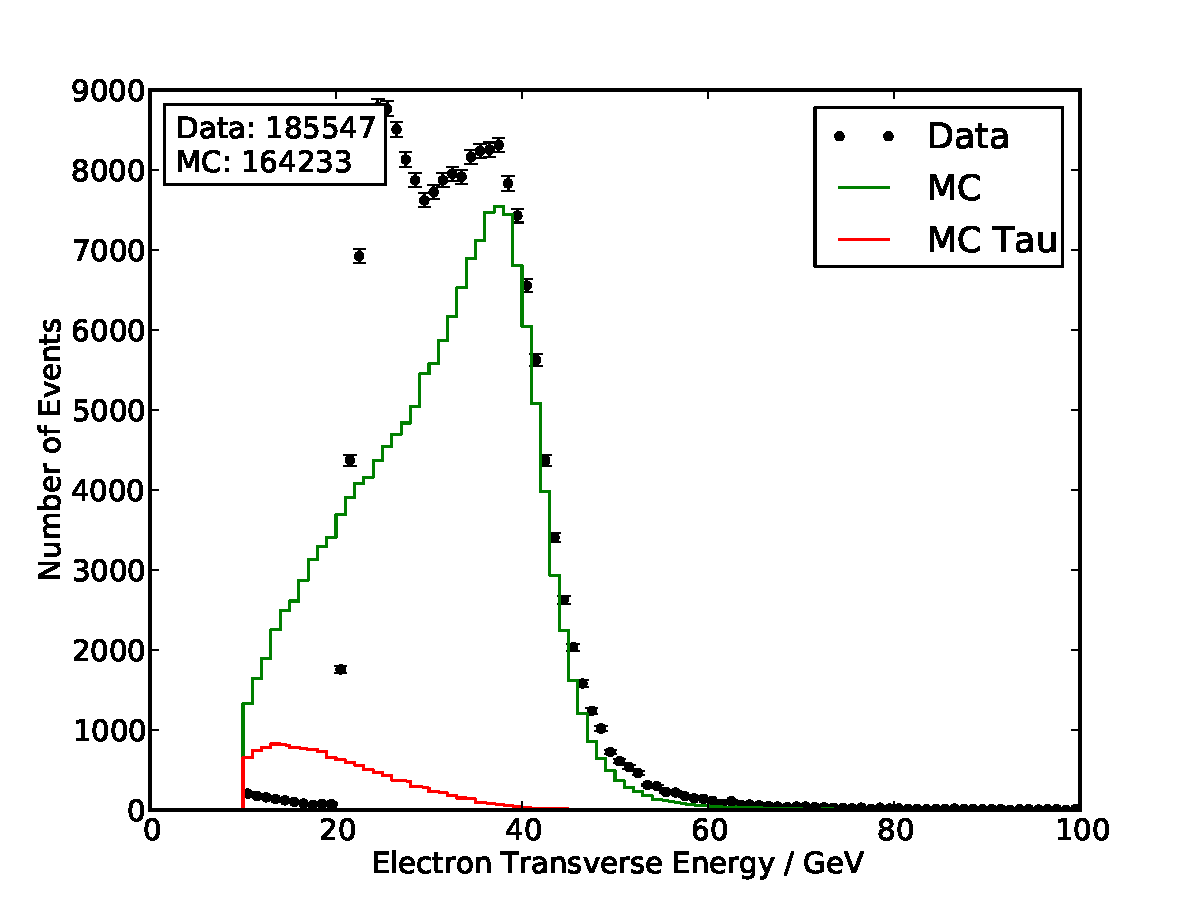
\includegraphics{nocuts/E_T_el}
		\caption{Transverse Electron Energy measured in the Central Calorimeter.}
	\end{subfigure}
	\begin{subfigure}{0.45\textwidth}
		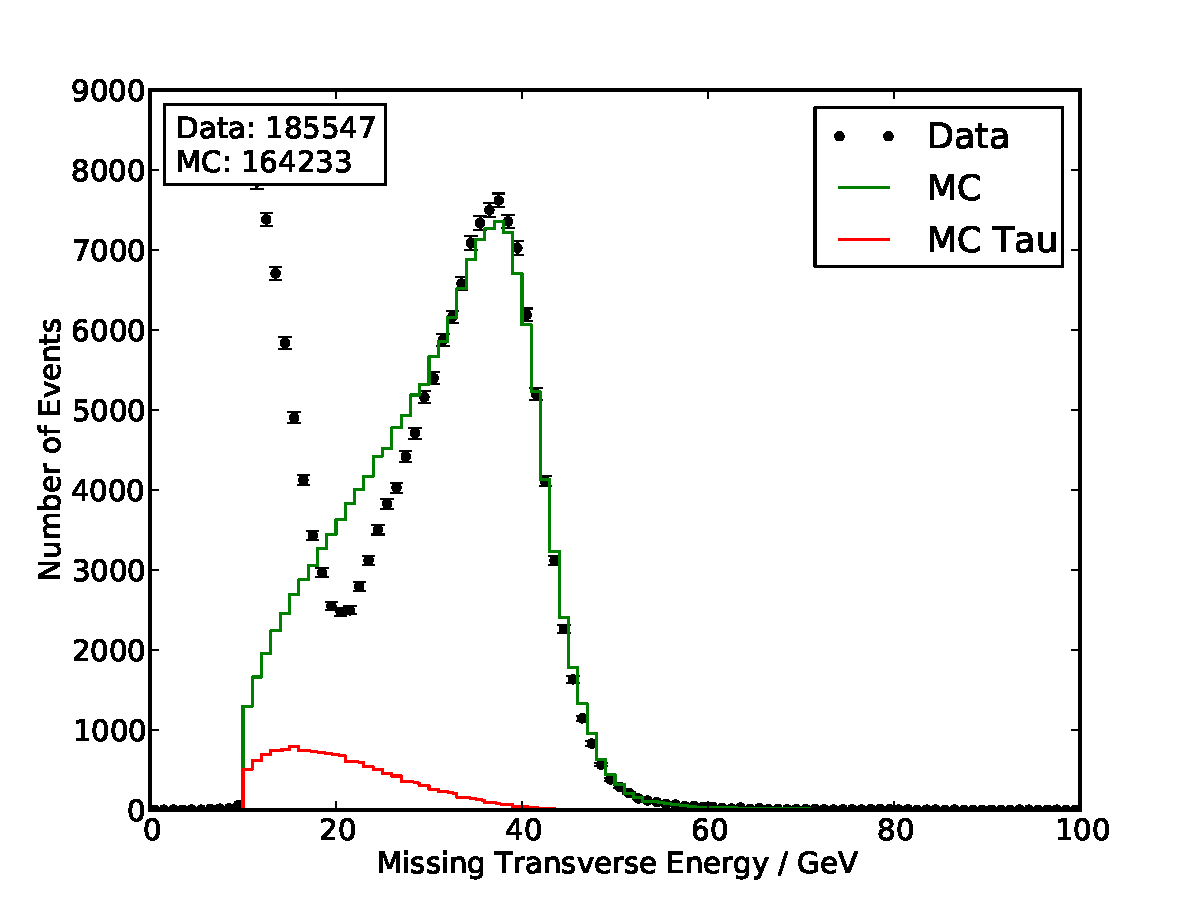
\includegraphics{nocuts/E_T_miss}
		\caption{Missing Transverse Energy, calculated using the constraint of momentum conservation in the transveral plane.}
	\end{subfigure}
	\caption{Distributions of Data and MC variables.}
	\label{fig:no_cuts_Etmet}
\end{figure}

\begin{figure}%
	\centering
	\begin{subfigure}{0.45\textwidth}
		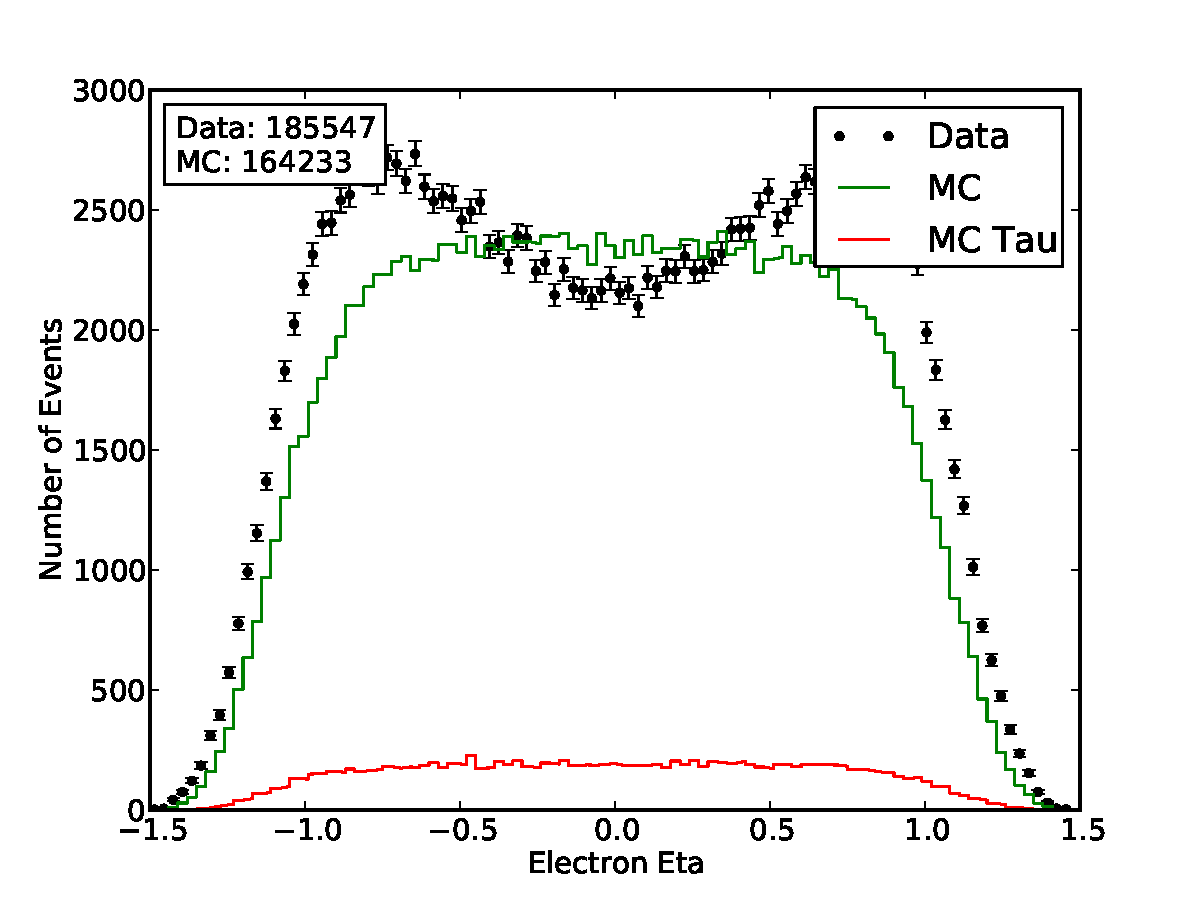
\includegraphics{nocuts/eta_el}
		\caption{Pseudorapidity of the Electron.}
	\end{subfigure}
	\begin{subfigure}{0.45\textwidth}
		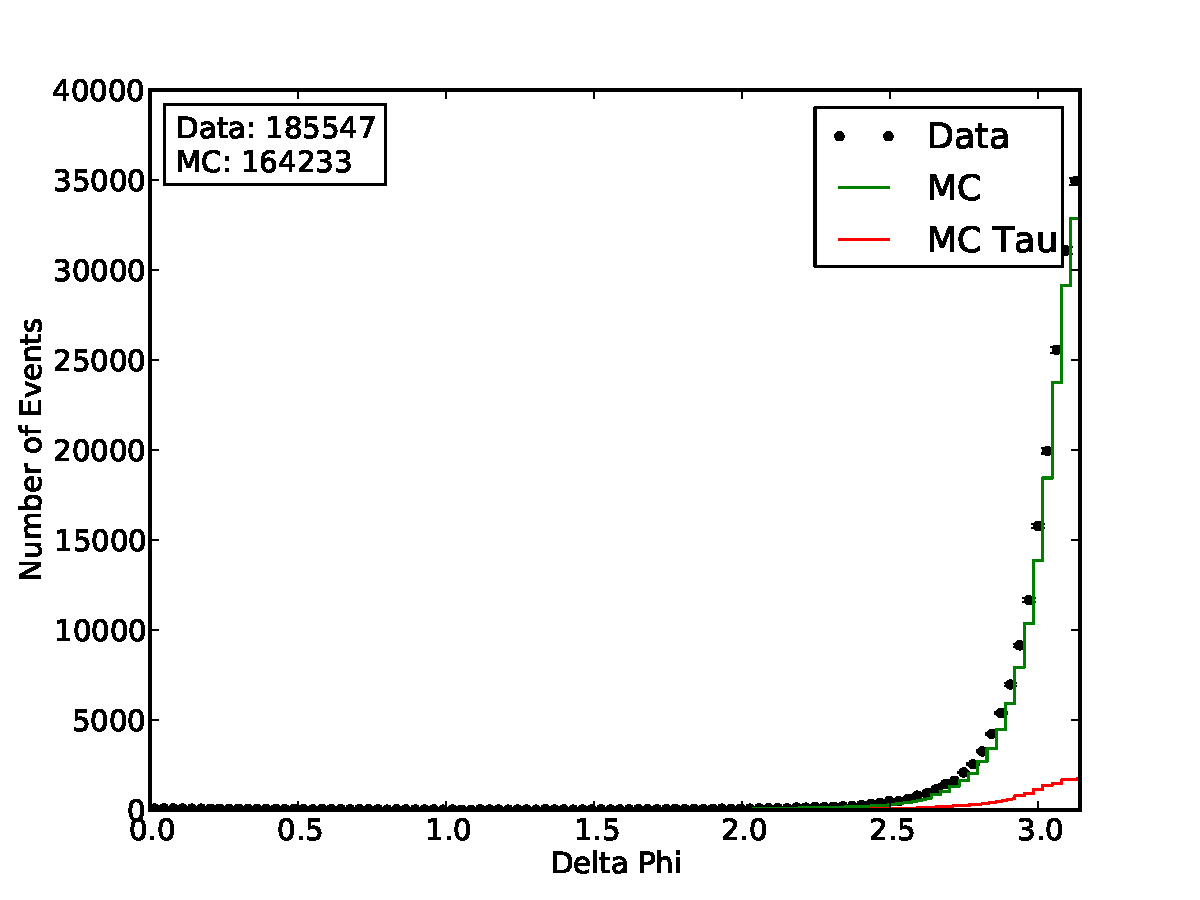
\includegraphics{nocuts/delta_phi}
		\caption{Difference in Polar Angle $\phi$ between the directions of MET and the electron.}
	\end{subfigure}
	\caption{Distributions of Data and MC variables.}
	\label{fig:no_cuts_etadphi}
\end{figure}

\begin{figure}%
	\centering
	\begin{subfigure}{0.45\textwidth}
		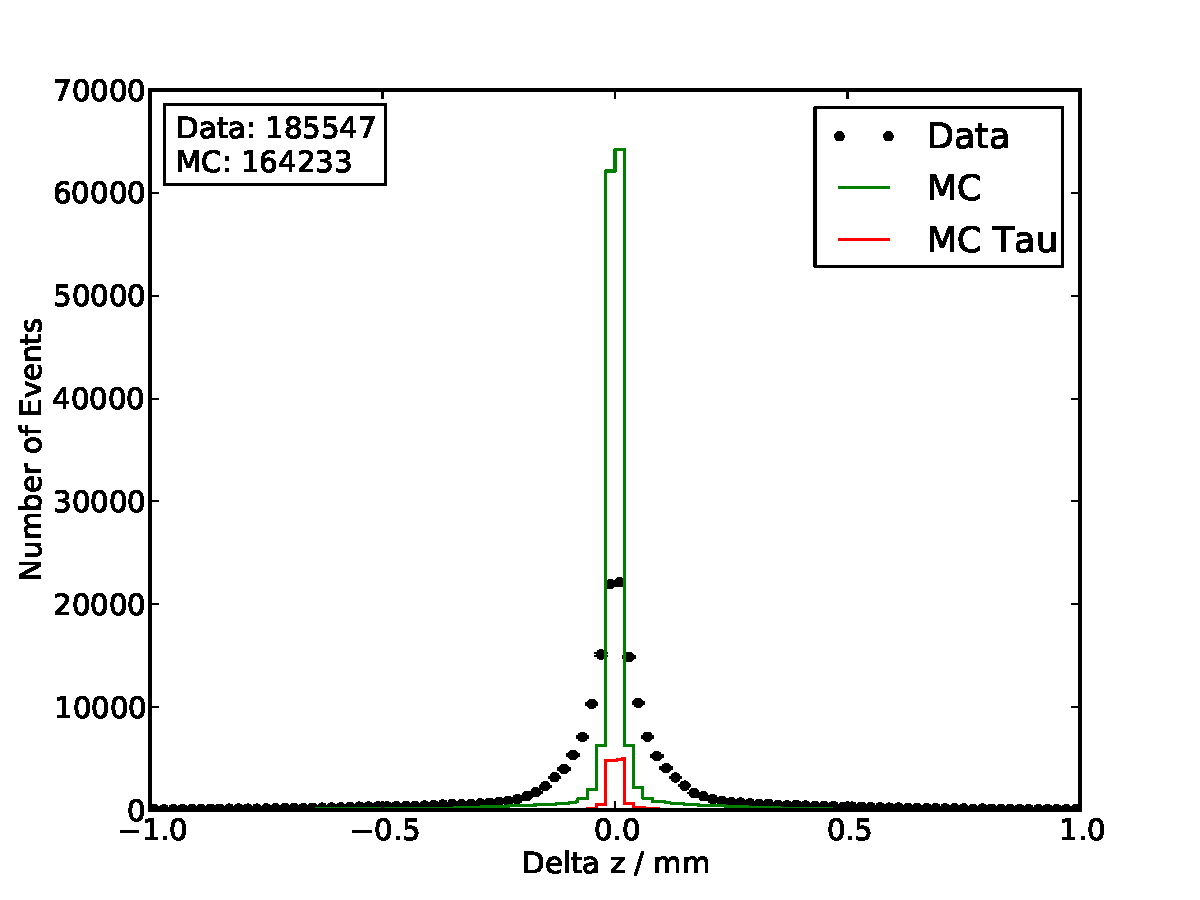
\includegraphics{nocuts/delta_z}
		\caption{Distance of the intersection point between MET and electron track to the collision point.}
	\end{subfigure}
	\begin{subfigure}{0.45\textwidth}
		%\includegraphics{Example}
		\caption{Isolation variable describing the tidiness in the vicinity of the electron's impact in the EM calorimeter}
	\end{subfigure}
	\caption{Distributions of Data and MC variables.}
	\label{fig:no_cuts_dziso}
\end{figure}

After applying these cuts, the agreement between data and MC becomes much better as can be seen in the distribution of the transverse electron energy (see figure \ref{fig:cuts_EtMt}). Since the reconstruction of the neutrino is only possible in the transverse plane of the detector, the invariant mass of the W-boson can not be calculated directly. The following analysis is therefore based on the transverse mass, which is calculated for each event:
\begin{equation}
M_t:=\sqrt{(p_T^{el}+p_T^{miss})^2} = \sqrt{\MET \ELET (1-\cos{\Delta \phi})}
\label{eq:m_t}
\end{equation} 
The distribution of this quantity is shown in figure \ref{fig:cuts_EtMt} and shows good agreement after applying the described cuts. Since rescaling of the MC events to the luminosity of the data sample as described in section \ref{ch:mc_samples} is very uncertain, the agreement of the absolute height is not very good. This discrepancy will not influence the main goal of the analysis and is therefore not investigated further. 

\begin{figure}%
	\centering
	\begin{subfigure}{0.45\textwidth}
		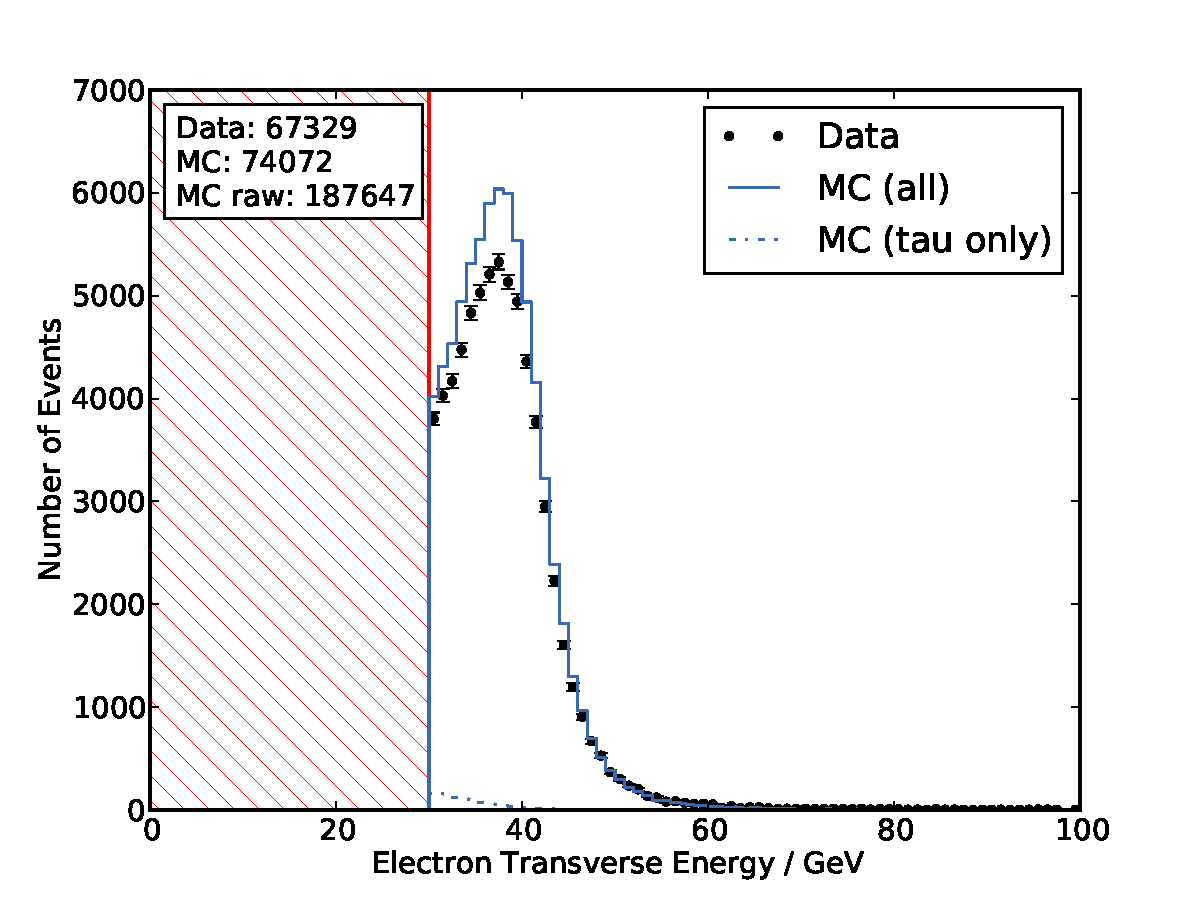
\includegraphics{allcuts/E_T_el}
		\caption{Transverse Electron Energy.}
	\end{subfigure}
	\begin{subfigure}{0.45\textwidth}
		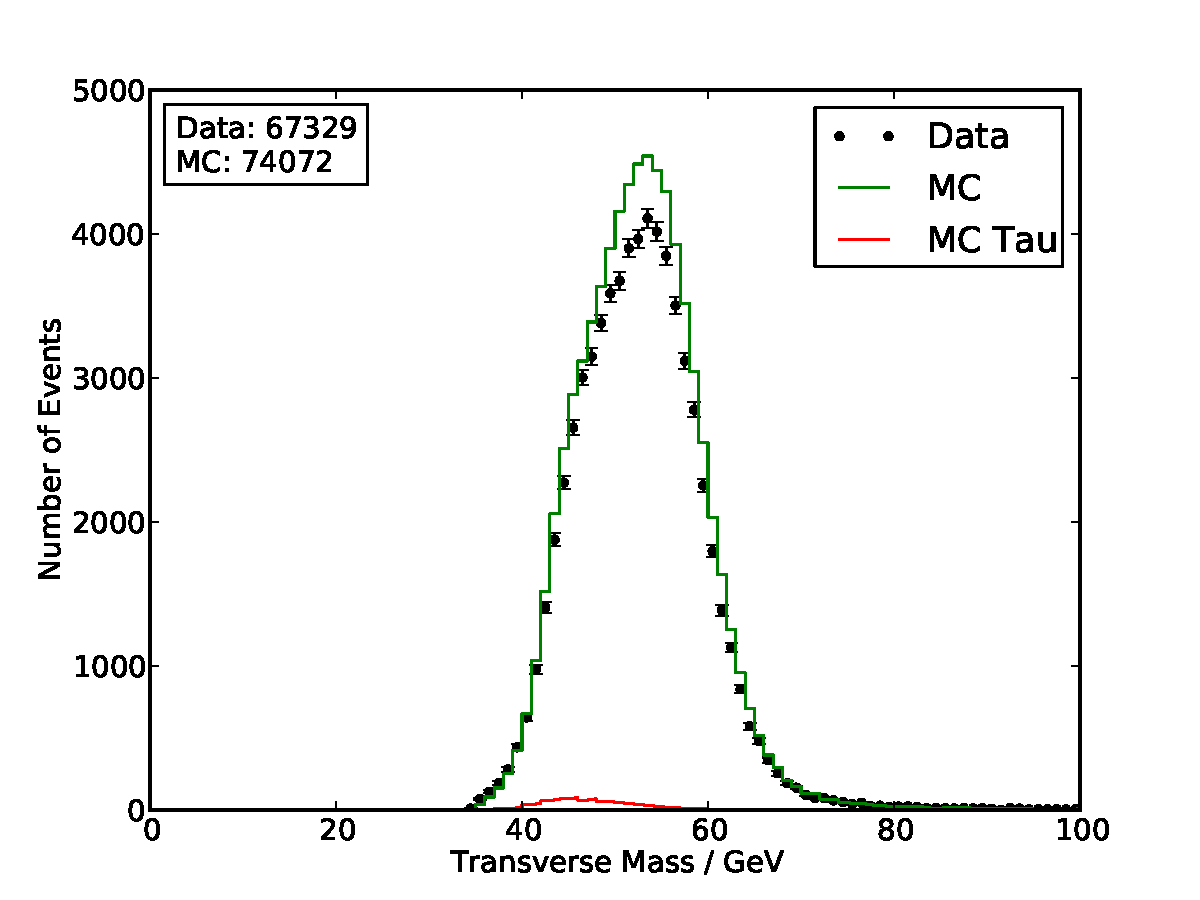
\includegraphics{allcuts/m_T}
		\caption{Reconstructed Transverse Mass.}
	\end{subfigure}
	\caption{Distributions of Data and MC variables, after applying the described cuts.}
	\label{fig:cuts_EtMt}
\end{figure}




\cleardoublepage

\bibliographystyle{utphys}
\bibliography{T17_bib}{}

\end{document}
